\subsubsection{Tensión de offset}

El cuadro \ref{tab:resultados-tension-offset} muestra las mediciones de tensión de offset.

\begin{table}[h!]
\centering
\begin{tabular}{|c|c|c|c|c|c|c|c|}
\hline
$V_o$ [V] & $\Delta V_o$ [V] & $R_f$ [K$\Omega$] & $\Delta R_f$ [K$\Omega$] & $R_s$ [$\Omega$] & $\Delta R_s$ [$\Omega$] & $V_{os}$ [mV] & $\Delta V_{os}$ [mV] \\ \hline
-8 & 0.4 & 100.000 & 5.000 & 100 & 5 & -8.000 & 0.690 \\ \hline
\end{tabular}
\caption{Mediciones de tensión de offset.}
\label{tab:resultados-tension-offset}
\end{table}

\subsubsection{Corriente de polarización Bias}

El cuadro \ref{tab:resultados-corriente-polarizacion} muestra las mediciones de las corrientes de polarización.

\begin{table}[h!]
\centering
\resizebox{\textwidth}{!}{  % Escala la tabla al ancho del texto
\begin{tabular}{|c|c|c|c|c|c|c|c|c|c|c|c|}
\hline
$V_o$ [V] & $\Delta V_o$ [V] & $R_f$ [$k\Omega$] & $\Delta R_f$ [$k\Omega$] & $R_s$ [$\Omega$] & $\Delta R_s$ [$\Omega$] & $R_b$ [$M\Omega$] & $\Delta R_b$ [$M\Omega$] & $V_{os}$ [mV] & $\Delta V_{os}$ [mV] & $I_B$ [nA] & $\Delta I_B$ [nA] \\ \hline
-8 & 0.4 & 100 & 5 & 100 & 5 & 22 & 1.1 & -8.000 & 0.690 & -0.00069 & 0.045 \\ \hline
8 & 1 & 100 & 5 & 100 & 5 & 22 & 1.1 & -8.000 & 0.690 & 0.73 & 0.071 \\ \hline
\end{tabular}
}
\caption{Mediciones de corriente de polarización.}
\label{tab:resultados-corriente-polarizacion}
\end{table}

El cuadro \ref{tab:resultados-corrientes-bias} muestra las mediciones de las corrientes $I_{B1}$, $I_{B2}$ e $I_{BIAS}$.

\begin{table}[h!]
\centering
\begin{tabular}{|c|c|c|c|c|c|}
\hline
$I_{B1}$ [nA] & $\Delta I_{B1}$ [nA] & $I_{B2}$ [nA] & $\Delta I_{B2}$ [nA] & $I_{BIAS}$ [nA] & $\Delta I_{BIAS}$ [nA] \\ \hline
-0.00069 & 0.045 & 0.73 & 0.071 & -0.73 & 0.084 \\ \hline
\end{tabular}
\caption{Mediciones de corrientes $I_{B1}$, $I_{B2}$ e $I_{BIAS}$.}
\label{tab:resultados-corrientes-bias}
\end{table}

\subsubsection{Mediciones del GBWP}

\begin{table}[h!]
\centering
\resizebox{\textwidth}{!}{
\begin{tabular}{|c|c|c|c|c|c|c|c|}
\hline
A & $\Delta$A & $f_l$ [Hz] & $\Delta f_l$ [Hz] & $f_h$ [kHz] & $\Delta f_h [kHz] $ & GBWP & $\Delta$GBWP [Hz] \\ \hline
100 & 7.86 & 2 & 0.8 & 7.14 & 0.051 & 714085.71 & 56335.44 \\ \hline
11.11 & 0.83 & 2 & 0.08 & 75.76 & 2.30 & 841728.62 & 67887.11 \\ \hline
1.00 & 0.08 & 2 & 0.08 & 892.86 & 31.89 & 892855.14 & 77056.50 \\ \hline
\end{tabular}
}
\caption{Mediciones del producto ganancia ancho de banda.}
\label{tab:resultados-gbwp}
\end{table}

\subsubsection{Mediciones del Slew Rate}

la figura \ref{fig:resultados-slew-rate} muestra la medición de la forma de onda del slew rate.

\begin{figure}[htbp]
\centering
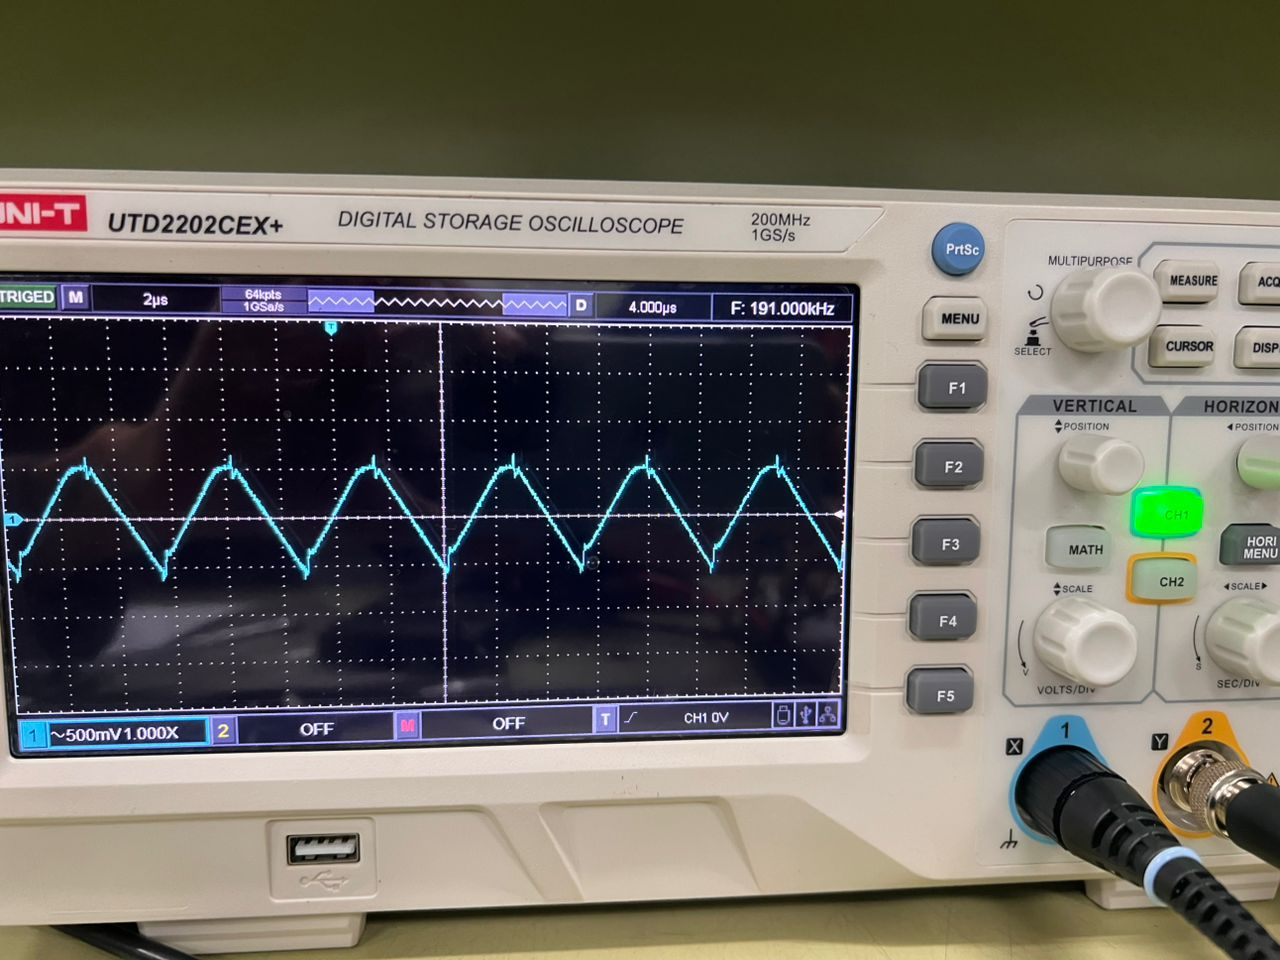
\includegraphics[width=0.5\textwidth]{resultados/slewrate.jpg}
\caption{Mediciones del slew rate.}
\label{fig:resultados-slew-rate}
\end{figure}

El cuadro \ref{tab:resultados-slew-rate} muestra las mediciones del slew rate.

\begin{table}[h!]
\centering
\begin{tabular}{|c|c|c|c|c|c|}
\hline
$V_o$ [V] & $\Delta V_o$ [V] & $\Delta t$ [$\mu$s] & $\Delta(\Delta t)$ [$\mu$s] & SR [V/$\mu$s] & $\Delta$SR [V/$\mu$s] \\ \hline
1 & 0.1 & 2 & 0.4 & 0.500 & 0.112 \\ \hline
\end{tabular}
\caption{Mediciones del slew rate.}
\label{tab:resultados-slew-rate}
\end{table}


\subsubsection{Mediciones de la corriente de cortocircuito}

\begin{table}[h!]
\centering
\begin{tabular}{|c|c|c|c|c|c|}
\hline
V [V] & $\Delta$V [V] & R [k$\Omega$] & $\Delta$R [k$\Omega$] & $I_{SC}$ [mA] & $\Delta I_{SC}$ [mA] \\ \hline
2.0 & 0.2 & 6.800 & 0.034 & 294.12 & 29.45 \\ \hline
\end{tabular}
\caption{Mediciones de la corriente de cortocircuito.}
\label{tab:resultados-corriente-cortocircuito}
\end{table}

El cuadro \ref{tab:resultados-corriente-cortocircuito} muestra las mediciones de la corriente de cortocircuito.




